\documentclass[10pt,t]{beamer}
\usetheme{Heverlee}

\newcommand\blfootnote[1]{%
  \begingroup
  \renewcommand\thefootnote{}\footnote{#1}%
  \addtocounter{footnote}{-1}%
  \endgroup
}

\usepackage{mathtools}
\usepackage{hyperref}
\usepackage{amsmath}
\usepackage{tikz}
\usepackage{overpic}
\usepackage{xcolor}

\newtagform{blank}{}{}
\usetagform{blank}

\newcommand{\lenitem}[2][0.45\linewidth]{\parbox[t]{#1}{\strut #2\strut}}

\renewcommand{\thefootnote}{[\arabic{footnote}]}
\AtBeginEnvironment{frame}{\setcounter{footnote}{0}}
\renewcommand{\theequation}{(\arabic{equation})}
\newcommand{\largecdot}{{\Large \;\boldsymbol{\cdot}\,}}

\setbeamertemplate{section in toc}
{\leavevmode\leftskip=2ex%
  \llap{%
    \usebeamerfont*{section number projected}%
    \usebeamercolor{section number projected}%
    \begin{pgfpicture}{2ex}{-0.5ex}{0ex}{0ex}
      \color{blue}
      \pgfpathcircle{\pgfpoint{0pt}{.75ex}}{1.7ex}
      \pgfusepath{fill}
      \pgftext[base]{\color{fg} \inserttocsectionnumber}
    \end{pgfpicture}\kern1.25ex%
  }%
~~{\large \color{blue} \inserttocsection\par}}

\definecolor{mygray}{gray}{.2}
\setbeamertemplate{subsection in toc}
{   
    \vspace{0.5em} 
    \leavevmode
    \leftskip=0.5em
    {\color{black} $-$}
    \hskip1em
    {\color{mygray} \inserttocsubsection}
    \par
}

\renewcommand{\mark}[1]{{\color{blue} \normalsize {#1}}}
\renewcommand{\emph}[1]{{\color{blue} {#1}}}

%%% QUICK OPTIONS:
% (A) Math font without serifs, enable line below to make math serif:
\usefonttheme[onlymath]{serif}
\setbeamerfont{itemize body}{size=\large} %block title font size
% \setbeamerfont{itemize subitem}{size=\large} %block title font size

% (B) Re-define primary colour by adjusting the RGB values
\definecolor{theme}{RGB}{0, 83, 159}   % The Udel color

% (C) Title page graphic (optional) --- this is not for the background image, see \usebackgroundtemplate to change that ---
% \titlegraphic{\includegraphics[height=2.7cm]{example_figure.pdf}}

% (D) Add logo to bottom right-corner (optional)
\logo{
\includegraphics[height=0.7cm]{Background/UDel-logo.jpg}}
% \logo{\includegraphics[height=0.6cm]{nju_logo.jpg}\hspace{12pt}\vspace{-6pt}}
% \logo{\includegraphics[height=0.5cm]{caltech_logo.png}\hspace{12pt}\vspace{-6pt}}   

% (E) Choose one (or none) of these lines to add footline bar on all frames
% \setbeamertemplate{footline}[infoline]  % author, title, insitute
% \setbeamertemplate{footline}[navigation] % dots swhowing progress
% \setbeamertemplate{footline}[navsym] % navigation symbols

% (F) Widescreen 16:9 ratio
\usepackage[orientation=landscape,size=custom,width=16,height=9,scale=0.45,debug]{beamerposter}
\usepackage{physics}
\newcommand{\nologo}{\setbeamertemplate{logo}{}}

%%% TITLE PAGE INFO:
\title{{\Large Markov chain Monte Carlo Simulation  \\
\vspace{0.5em} An Example with Argon}}
\author{Astolfo}
\date{\today}

% Text inside {} is used on the title page. Text inside [] is optional, and is used in footline bar (if [] is omitted then text from {} will be used in both ; if [] is specified but left empty then the footline will not show any text)

\begin{document}
 %%
 %%  0. TITLE PAGE and TABLE OF CONTENT
 %%
% Title page

{
% Change image, or delete this line to remove background image
%  %   abudhabi      cherry      forest      river
%  %   alishan       chobe       leuven      sanfancisco
%  %   blueprint     columns     library     uyuni
%  %   bokeh         flowers     newyork     winter

\setbeamercolor{background canvas}{bg=lgray}
% make background light gray
\begin{frame}[plain,noframenumbering]
    \titlepage
\end{frame}
}

% Table of contents slide
\begin{frame}{Outline}
\hfill {\parbox{1.0\textwidth}{\tableofcontents[hideothersubsections]}}
\end{frame}

\section{Introduction}

{
\begin{frame}
\frametitle{Brief introduction to Markov chain Monte Carlo}
\begin{itemize}
\vspace{-0.6em}
\setlength\itemsep{1em}
    \item For equilibrium distribution, the average of a physical quantity
$A$ in equilibrium is
    \begin{equation*}
        \langle A \rangle = \int \dd \mathbf{x} \dd \mathbf{p} \, \rho(\mathbf{x},\mathbf{p}) A(\mathbf{x},\mathbf{p})
    \end{equation*}
    Here, $\rho(\mathbf{x},\mathbf{p}) = e^{-\beta H(\mathbf{x},\mathbf{p})}/Z$ is the canonical ensemble distribution function, and $Z = \int d\mathbf{x}  \dd \mathbf{p} \, e^{-\beta H(\mathbf{x},\mathbf{p})}$ is the canonical partition function.
    \item Classically, momentum $\mathbf{p}$ and position $\mathbf{x}$ can be obtained simultaneously, which means $\langle e^{-\beta H(\mathbf{x},\mathbf{p})}\rangle=\langle e^{-\beta T(\mathbf{p})} \rangle \langle e^{-\beta U(\mathbf{x})}\rangle$, and if $A$ only depends on $\mathbf{x}$, we have
    \begin{equation*}
        \langle A \rangle = \int \dd \mathbf{x} \, \rho(\mathbf{x}) A(\mathbf{x})
    \end{equation*}
    Here, $\rho(\mathbf{x}) = e^{-\beta U(\mathbf{x})}/Z$ and $Z = \int d\mathbf{x} \, e^{-\beta U(\mathbf{x})}$ only depends on $\mathbf{x}$.
\end{itemize}
\end{frame}
}

{
\begin{frame}
\frametitle{Detailed balance}
\begin{itemize}
\vspace{-0.6em}
\setlength\itemsep{1em}
    \item When equilibrium, the probability of the system being in configuration $\mathbf{x}_a$ do \\ not change with time. Therefore, we have
$$
\dv{\rho_a}{t} = \sum_b \left[ w_{b \to a} \rho_b - w_{a \to b} \rho_a \right] = 0
$$
Here, $w_{b \to a}$ represents the transition probability from configuration $\mathbf{x}_b$ to $\mathbf{x}_a$. 

\item From the above relation, we can deduce that if \textbf{detailed balance} is satisfied,\\ we can generate a sequence that follows the Boltzmann distribution
$$
\frac{w_{a \to b}}{w_{b \to a}} = \frac{\rho_b}{\rho_a} = e^{-\beta (E_b - E_a)} = e^{\beta \Delta E_{ab}}
$$
\end{itemize}
\end{frame}
}

{
\begin{frame}
\frametitle{Metropolis–Hastings algorithm}
\begin{itemize}
\vspace{-0.6em}
\setlength\itemsep{1em}
    \item Metropolis transition probability
$$\left.w_{a\to b}=\left\{\begin{array}{cc}e^{\beta\Delta E_{ab}}&(E_b>E_a)\\1&(E_b\leq E_a)\end{array}\right.\right.$$

\item Metropolis–Hastings algorithm \\
1. Initial configuration $\mathbf{x}_{i}$ with energy $E_{i}$;\\
2. Random move to a new configuration $\mathbf{x}_{i'}$ with energy $E_{i'}$;\\
3. If $E_{i'}\leq E_{i}$ or $e^{\beta (E_{i'}-E_{i})} < R$, $R$ is random number in $[0,1)$, accept the move. The next configuration will be $\mathbf{x}_{i+1} = \mathbf{x}_{i'}$;\\
4. Return to step 2 and repeat until $N$ configurations have been accumulated.\\

\item Starting from any initial configuration, the system will eventually reach equilibrium and follow the Boltzmann distribution. 
\end{itemize}
\end{frame}
}

\section{Simulation system setup}
\begin{frame}
    \frametitle{Argon}
    \begin{itemize}
    \vspace{-0.6em}
    \setlength\itemsep{1em}
        \item Argon is a chemical element; it has symbol Ar and atomic number 18. It is in group 18 of the periodic table and is a noble gas.       
        \item Melting point: 83.81 K, boiling point: 87.302 K, triple point: 83.8058 K
        \item Liquid density (at b.p.): 0.02103 \AA$^{-3}$
        \item Lattice: FCC (a=5.4691 \AA), density: 0.02445 \AA$^{-3}$ (at triple point)
    \end{itemize}
    \begin{figure} % [htbp]
        \centering
        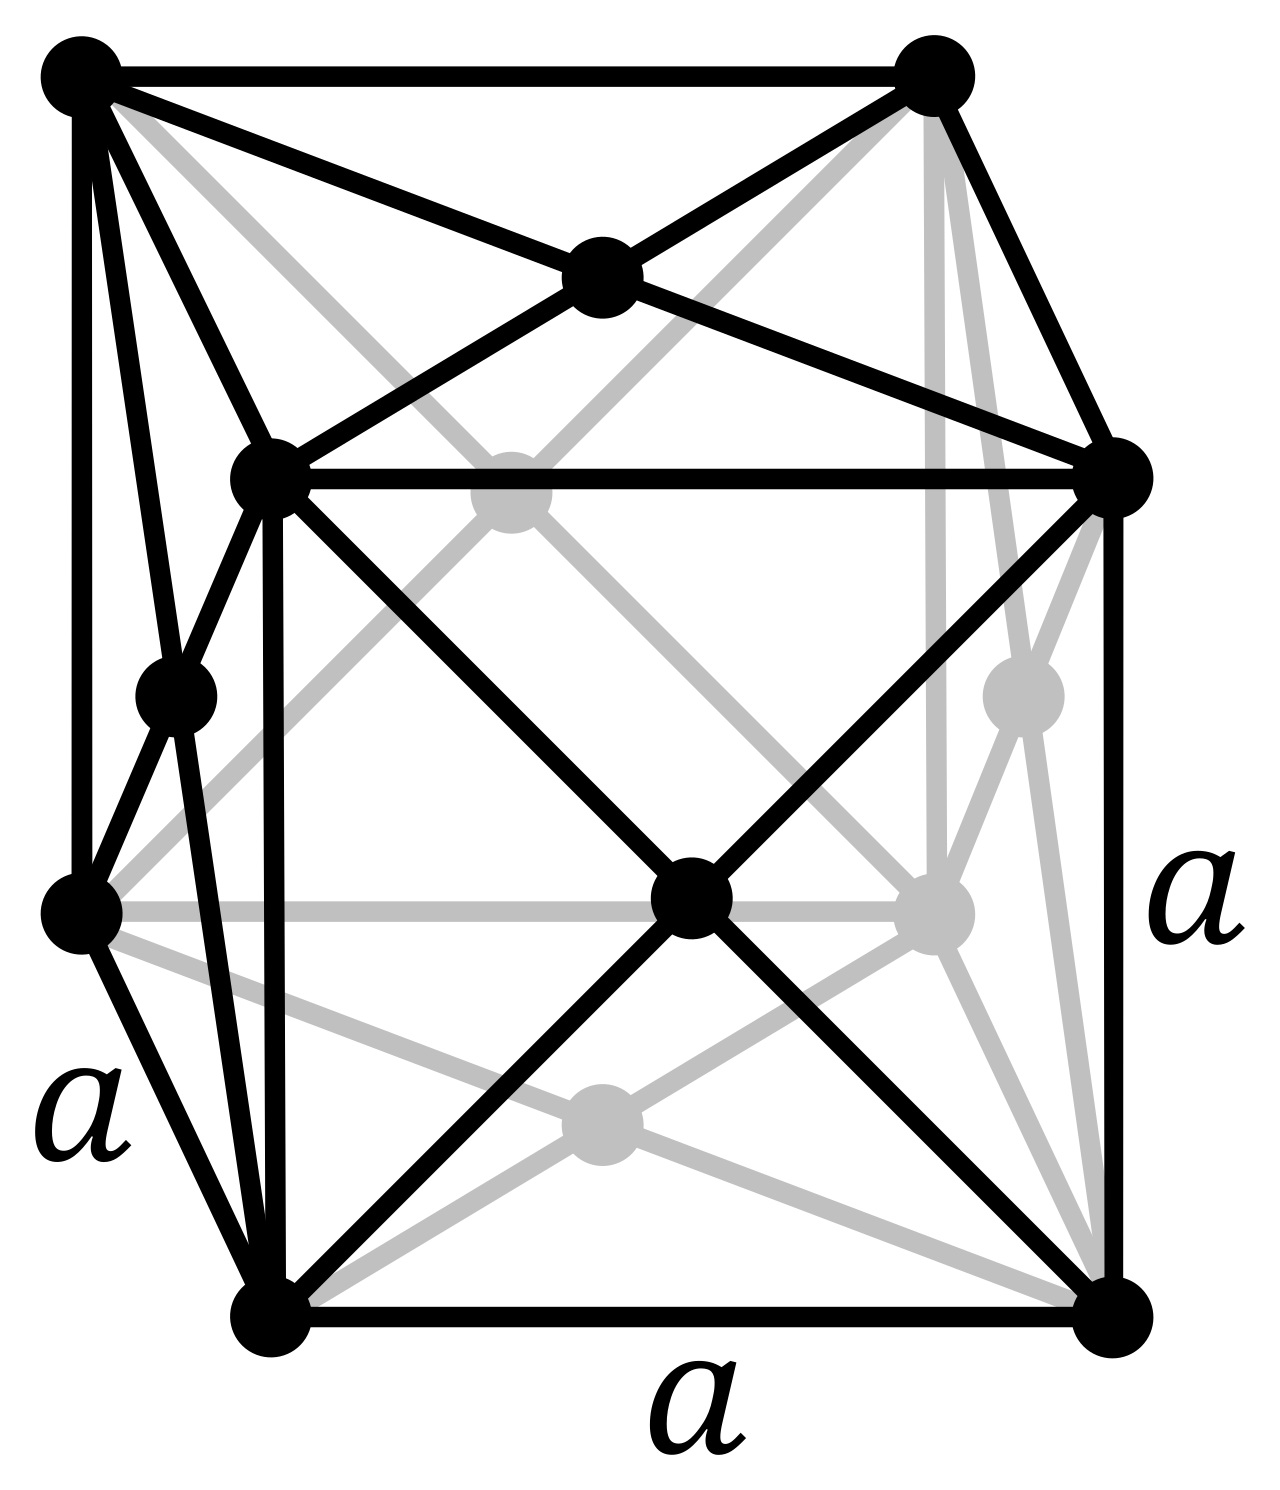
\includegraphics[width=0.15\textwidth]{figures/Cubic-face-centered.png} 
    \end{figure}
\end{frame}

\begin{frame}
\frametitle{Mie potential}
\begin{itemize}
\vspace{-0.6em}
\setlength\itemsep{1em}
    \item Mie potential is an interaction potential describing the interactions between particles on the atomic level. It is mostly used for describing intermolecular interactions, but at times also for modeling intramolecular interaction.
    \begin{equation*}
        U(r) = C \varepsilon \left[\left(\frac{\sigma}{r}\right)^n-\left(\frac{\sigma}{r}\right)^m\right]
    \end{equation*}
    with
    \begin{equation*}
        C = \frac{n}{n-m}\left(\frac{n}{m}\right)^{\frac{m}{n-m}}
    \end{equation*}
    \item The Lennard-Jones potential corresponds to the case where n=12 and m=6.
    \item For Ar, $\sigma$=3.404 \AA, $\varepsilon$=117.84 $k_B$, n=12.085, m=6.0.
\end{itemize}
\end{frame}

\section{Results and conclusion}
\begin{frame}
    \frametitle{Pair correlation function}
    \begin{itemize}
    \vspace{-0.6em}
    \setlength\itemsep{1em}
        \item Pair correlation function $g(r)$ in a system of particles describes how density varies as a function of distance from a reference particle.
        \begin{equation*} g(\mathbf{r}_1,\mathbf{r}_2)=\frac{\rho(\mathbf{r}_1,\mathbf{r}_2)}{\rho(\mathbf{r})^2}
        \end{equation*}
        In fluid, $\rho(\mathbf{r})=\rho$, $g(\mathbf{r}_1,\mathbf{r}_2)=g(|\mathbf{r}_1-\mathbf{r}_2|)\equiv g(r)$. $g(r)$ can also be referred to as the radial distribution function. When $r \to +\infty$, $g(r) \to 1$.
        \item In practice, we choose a series of radius grids $\{r_i\}$, which have the same difference $\dd r$, and the pair correlation function can be calculated using
        \begin{equation*} 
        g(r_i)=\frac{1}{\rho}\frac{n(r_i)}{4 \pi r_i^2 \dd r}
        \end{equation*}
    \end{itemize}
\end{frame}

\begin{frame}
    \frametitle{Liquid case}
    \begin{itemize}
    \vspace{-0.6em}
    \setlength\itemsep{1em}
        \item Density : 0.02103 \AA$^{-3}$, Tempreature: 84K
        \item nmol: 108, box: $3 \times 3 \times 3$ unit cell, $a_0$ is box size, ncycle: 1000, ngrid: 100.
    \end{itemize}
    \begin{figure} % [htbp]
        \centering
        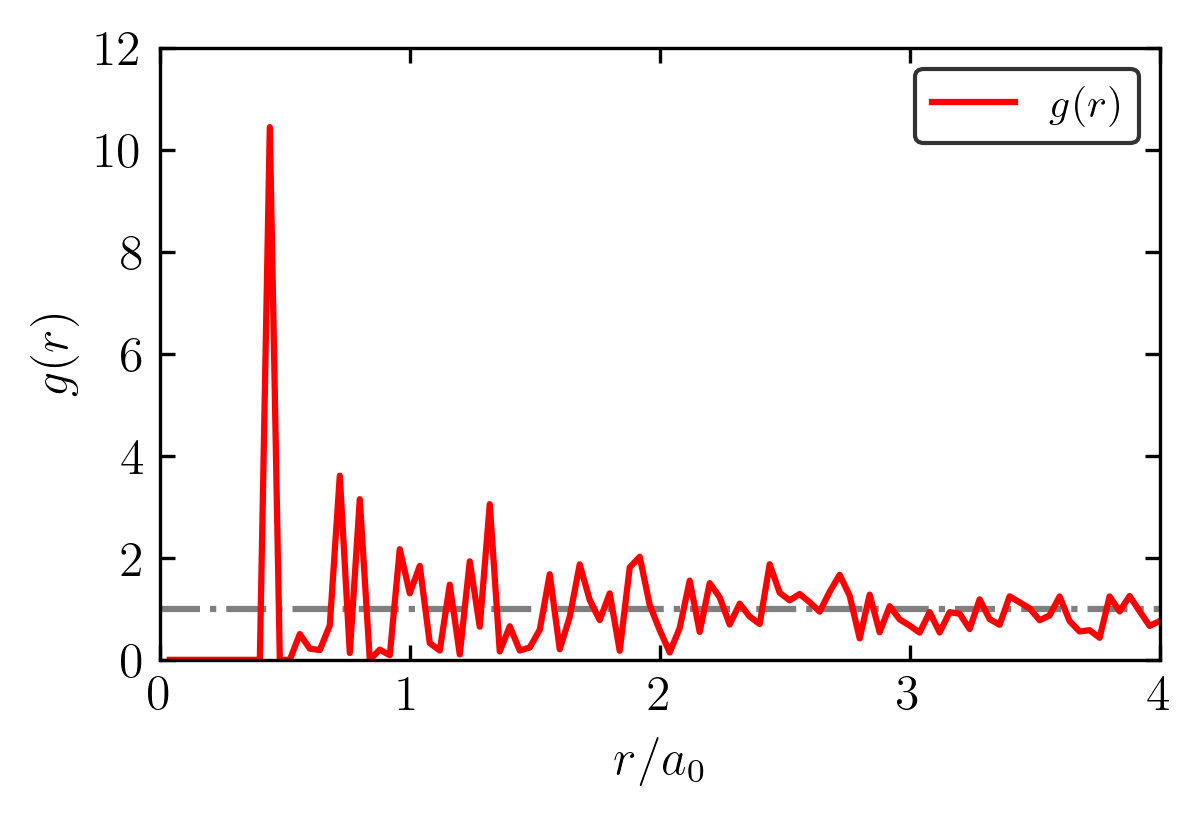
\includegraphics[width=0.5\textwidth]{figures/Ar_84K_333.png} 
    \end{figure}
\end{frame}

\begin{frame}
    \frametitle{Solid case}
    \begin{itemize}
    \vspace{-0.6em}
    \setlength\itemsep{1em}
        \item Density : 0.2103 \AA$^{-3}$, Tempreature: 10K
        \item nmol: 108, box: $3 \times 3 \times 3$ unit cell, $a_0$ is box size, ncycle: 1000, ngrid: 100.
    \end{itemize}
    \begin{figure} % [htbp]
        \centering
        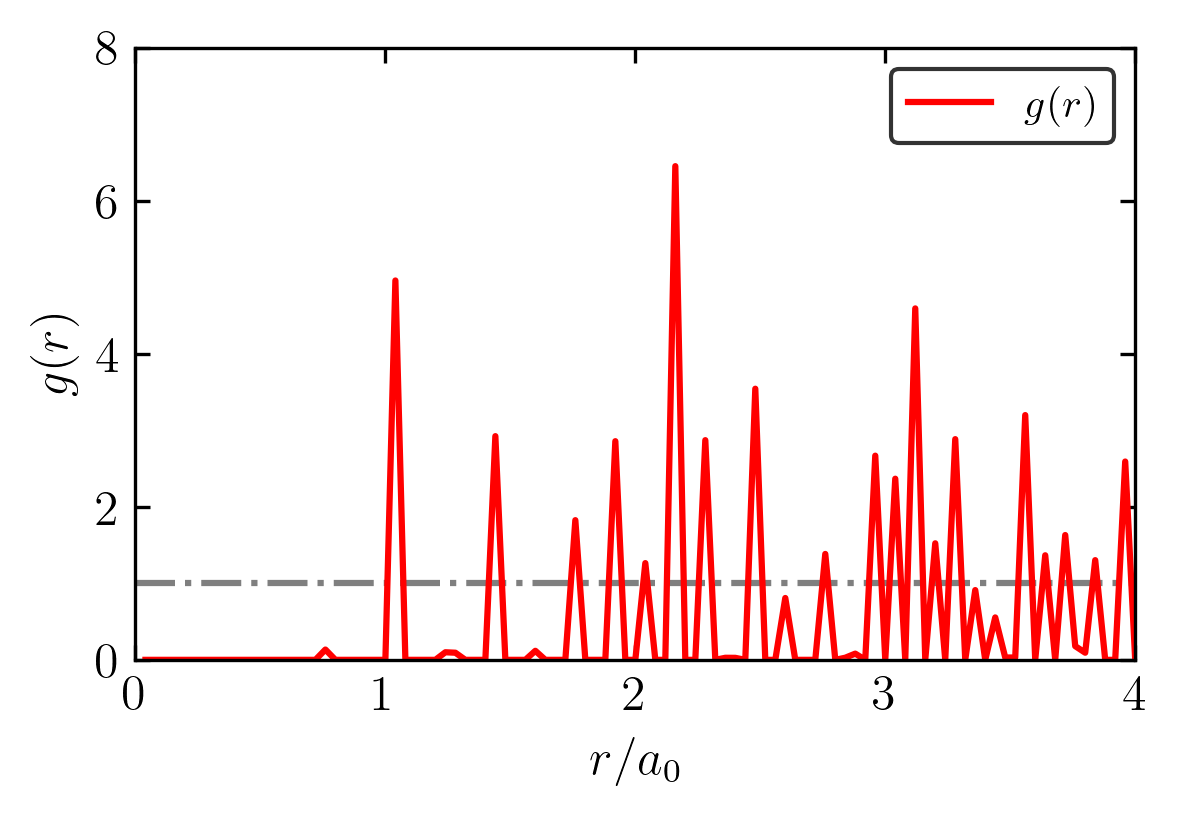
\includegraphics[width=0.5\textwidth]{figures/Ar_10K_333_high.png} 
    \end{figure}
\end{frame}

\begin{frame}
    \frametitle{Why higher density}
    \begin{itemize}
    \vspace{-0.6em}
    \setlength\itemsep{1em}
        \item Density : 0.02445 \AA$^{-3}$, Tempreature: 10K
        \item nmol: 108, box: $3 \times 3 \times 3$ unit cell, $a_0$ is box size, ncycle: 1000, ngrid: 100.
    \end{itemize}
    \begin{figure} % [htbp]
        \centering
        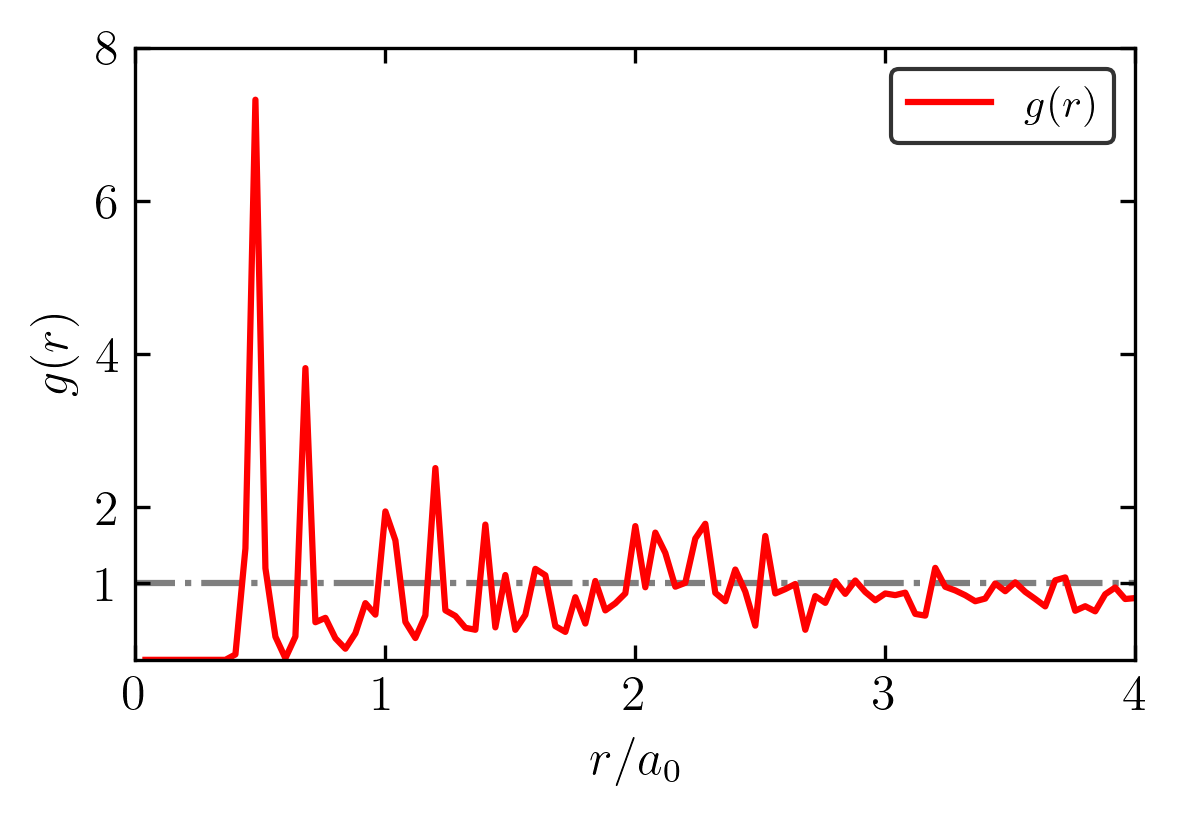
\includegraphics[width=0.5\textwidth]{figures/Ar_10K_333.png} 
    \end{figure}
\end{frame}

\begin{frame}
    \frametitle{Conclusion}
    \begin{itemize}
    \vspace{-0.6em}
    \setlength\itemsep{1em}
        \item Mie potential is used to describe the potential of a fluid, and is not applicable \\ for solids. In this case, only by applying sufficiently large pressure to the system can some solid-like properties be exhibited.
        \item The radius of the first peak in the three graphs, when converted to \AA, is approximately the same (3.4506 \AA, 3.2031 \AA, 3.2814 \AA) around the equilibrium position of the potential  ($\sigma = 3.404$ \AA).
    \end{itemize}
\end{frame}

\end{document}


